\cleardoublepage
\appendix
\chapter{Hướng dẫn sử dụng phần mở rộng Burp Suite}
Trong trường hợp lần đầu sử dụng ứng dụng, ta cần cài đặt phần mở rộng \texttt{y4t0g4m1.jar} trong đường dẫn gốc của mã nguồn backend vào công cụ Burp Suite. Chi tiết việc cài đặt thêm phần mở rộng Java có thể tham khảo tại \parencite{burp-suite-extension-setup}. Giao diện chính của phần mở rộng trên Burp Suite được mô tả như Hình \ref{fig:main-burp-extension-interface} dưới đây, chỉ đơn giản gồm một textbox để thiết lập địa chỉ máy chủ ứng dụng nhận request mẫu. Mặc định giá trị của trường này là \texttt{http://61.28.235.183:13336}, là địa chỉ backend ứng dụng được triển khai trên \acrshort{vps} với cổng mặc định là 13336. \acrshort{ui} của webfuzzer hiện đang được triển khai trên đường dẫn \texttt{http://61.28.235.183:3000}.
\begin{figure}[H]
  \centering
    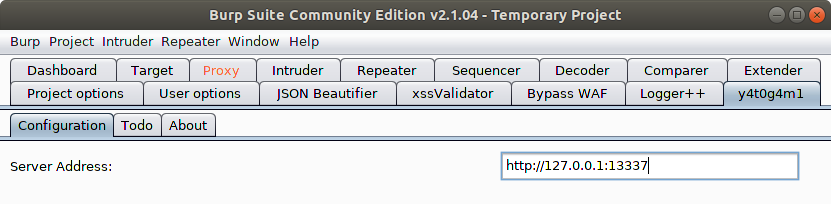
\includegraphics[width=\textwidth,keepaspectratio=true]{images/main-burp-extension-interface.png}
  \caption{Giao diện chính của phần mở rộng trên Burp Suite}
  \label{fig:main-burp-extension-interface}
\end{figure}
Sau khi khởi chạy \acrshort{ui} của ứng dụng webfuzzer và cài đặt phần mở rộng trên Burp Suite, ta tiến hành thiết lập proxy trên Burp Suite và trình duyệt web để bắt request mẫu như hướng dẫn tại \parencite{burp-suite-proxy}. Sau đó ta chuyển request mong muốn đến tab \texttt{Intruder} để tạo và gửi request mẫu đến máy chủ webfuzzer. Hình \ref{fig:send-base-request-1} mô tả quá trình này bằng cách thêm hoặc bỏ các kí tự ``\texttt{\S}'' bao quanh giá trị của tham số và chọn ``\texttt{Send to y4t0g4m1 webfuzzer}''. Request mẫu này sau đó sẽ hiển thị trên khung danh sách request mẫu ở trang bảng điều khiển của \acrshort{ui} ứng dụng webfuzzer để người dùng tiến hành chọn lỗ hổng và kiểm thử.